\chapter[Proposta de viabilização]{PROPOSTA DE VIABILIZAÇÃO}

\section{Solução do Sistema Embarcado}

Para o sistema embarcado será desenvolvido um algoritmo para realizar o processamento de imagem, para identificação de faixa de pedestre. Para esse projeto utilizaremos a placa Raspberry Pi que possui todos os recursos necessários para o desenvolvimento dos requisitos e capaz de realizar um processamento de imagem com qualidade.

\begin{figure}[h]
\includegraphics[scale=0.2]{figuras/Capitulo4/rasp.jpg}
\centering
\caption{Raspberry Pi.}
\label{fig:rasp.jpg}
Fonte: \cite{rasp}
\end{figure}

Para a realização do processamento de imagem usaremos a Pi.camera pelo seu tamanho compacto e de fácil utilização quando acoplado a raspberry.
\begin{figure}[h]
\includegraphics[scale=0.2]{figuras/Capitulo4/camera.jpg}
\centering
\caption{Pi câmera.}
\label{fig:camera.jpg}
Fonte: \cite{camera}
\end{figure}

Já para a realização do controle de todo o sensoriamento utilizaremos outro microcontrolador sendo ele responsável, pelo controle de todos os sensores ultrassônicos e de todos os vibracalls presente. Sendo de fundamental importância para a localização do deficiente visual. Desenvolveremos o algoritmo nesse recurso pelo seu tamanho reduzido facilitando assim a implementação na estrutura e devido ao seu consumo de corrente sendo bem menor aumentando assim a durabilidade da bateria.

\begin{figure}[h]
\includegraphics[scale=0.4]{figuras/Capitulo4/msp.png}
\centering
\caption{Microcontrolador MSP430.}
\label{fig:msp.png}
Fonte: \cite{msp}
\end{figure}

Na realização do sensoriamento serão utilizados sensores HC-SR04, sensores ultrassônicos, responsáveis por medir a proximidade do deficiente visual com obstáculos. Seu princípio de funcionamento está baseado na emissão de uma onda sonora de alta frequência, e na medição do tempo levado para a recepção do eco produzido quando esta onda se choca com o objeto.

\begin{figure}[h]
\includegraphics[scale=0.8]{figuras/Capitulo4/sensor.JPG}
\centering
\caption{Sensor Ultrassônico.}
\label{fig:sensor.jpg}
Fonte: \cite{sensor}
\end{figure}

\section{Sistema de Alimentação}

O SmartWay terá um sistema de alimentação independente com baterias que possa ser recarregado de maneira  rápida, fácil e adaptado às necessidades do usuário, por isso, será necessário um sistema que tenha um aviso sonoro indicando as baterias estão descarregadas. 

A partir de pesquisa e entrevistas com deficientes visuais, foi concluído que um aspecto relevante para a adaptação a esse tipo de tecnologia é o tempo de autonomia do sistema, que normalmente é abaixo da quantidade de horas necessárias diariamente do usuário. Economia de energia em todas os módulos do processo deverá ser feita para atender esse fim, além da escolhas de baterias que tenha uma bom tempo de autonomia de acordo com a carga do sistema.

Além disso, o peso e dimensão do sistema são aspectos que devem ser considerados. O peso deve ser o menor possível visto que um equipamento pesado teria um difícil adaptação para o uso constante durante caminhadas. A dimensão física deve ser adequada ao design da bengala e ao modelo que for confortável durante o uso.

Como solução, a bateria escolhida para alimentar a Raspberry Pi será uma bateria recarregável Li-Ion. As vantagens sobre os outros tipos de bateria são: peso leve e alta de capacidade de carga. Além disso a bateria de íons de lítio não tem efeito memória, ou seja, não vicia, logo,  não é preciso carregar a bateria até o total da capacidade e descarregar até o total mínimo.
	

\section{Solução de Estrutura}

Para a estrutura, o caminho inicial foi pensado para que o produto desenvolvido seja o mais próximo possível da bengala para deficientes visuais utilizada atualmente. Isso se deve ao fato de que o mesmo poderá ser utilizado tanto com os sistemas ativos, quanto com sistemas inativos, em caso de bateria fraca ou mesmo a não necessidade do sistema. Deve-se também à necessidade de proporcionar conforto ao usuário, uma vez que a bengala existente possui formatos anatômicos que se enquadram ao cotidiano do deficiente visual.

Inicialmente, o dispositivo deve conter todas as partes do sistema embarcado em seu interior. A partir deste requisito, desenvolveu-se um estudo a respeito da disposição dos subsistemas ao longo da bengala, de forma que suas características anatômicas e sensoriais originais fossem mantidas.

\begin{figure}[H]
\includegraphics[scale=2]{figuras/bengala/bengala.jpg}
\centering
\caption{Bengala original}
\label{fig:sensor.jpg}
\end{figure}

A bengala para deficientes visuais original possui uma distribuição de peso que deve ser mantida, em proporção, no dispositivo desenvolvido, ou seja, o sistema embarcado deve estar disposto de forma a se aproximar ao máximo do posicionamento do centro de massa da bengala convencional.

A partir dos requisitos propostos para o funcionamento da eletrônica juntamente com os requisitos anatômicos, o dispositivo será confeccionado utilizando tubos de seção transversal circular de material compósito, o sistema de alimentação ficará posicionado atrás da manopla onde a mão do usuário estará, a Raspberry Pi ficará posicionada logo a frente deste mesmo ponto, juntamente com o primeiro sensor ultrassônico. O segundo sensor ultrassônico será posicionado 60 centímetros abaixo do primeiro.

\begin{figure}[H]
\includegraphics[scale=0.5]{figuras/bengala/bengalacompleta.PNG}
\centering
\caption{CAD da Bengala completa}
\label{fig:sensor.jpg}
\end{figure}

Para acomodar a Raspberry Pi e o primeiro sensor ultrassônico, será feita uma modificação do formato da seção transversal do tubo original, de forma a deformar apenas o necessário no formato original do tubo, visando permanecer visual e anatomicamente próxima ao dispositivo tradicional. Os componentes eletrônicos necessitam de dissipação de calor para que permaneçam funcionando normalmente, portanto, será utilizada chapa de alumínio como parte da estrutura da seção portadora da Raspberry Pi, de forma que a mesma mantenha contato com o metal, não necessitando da abertura de uma janela de ventilação. Da mesma forma o segundo sensor ultrassônico será alocado sendo deformada a seção transversal do ponto onde deverá se posicionar.

\begin{figure}[H]
\includegraphics[scale=0.5]{figuras/bengala/conexaobengalacorreto.PNG}
\centering
\caption{CAD das conexões da bengala}
\label{fig:sensor.jpg}
\end{figure}

\begin{figure}[H]
\includegraphics[scale=0.5]{figuras/bengala/senssorultrassonico2.PNG}
\centering
\caption{CAD do sonar}
\label{fig:sensor.jpg}
\end{figure}


Por necessitar ser portátil, a mesma será desmontável em quatro partes de mesmo comprimento, contando com junções projetadas para serem intuitívas e práticas, não necessitando encaixe. A junção é formada por uma interrupção na sessão transversal da bengala, obtendo-se duas paredes, uma em cada extremidade seccionada. Estas paredes possuirão ímãs de neodímio posicionados de forma a se atrairem ao aproximar-se os dois extremos para a posição correta, sem a necessidade de ser posicionado da maneira correta pelo usuário. Após este posicionamento magnético, o usuário puxará logo abaixo uma luva externa ao tubo que conta com engate rápido no tubo superior, para que a mesma seja travada e sua rigidez mantida para o uso devido. Para desmontar, basta baixar a luva e dobrar a bengala como desejar.

\begin{figure}[H]
\includegraphics[scale=0.5]{figuras/bengala/eletronicacorreto.PNG}
\centering
\caption{CAD da Bengala com parte eletrônica discretizada}
\label{fig:sensor.jpg}
Fonte: \cite{sensor}
\end{figure}


\section{Solução de Software}

A solução proposta pela equipe de software é que mediante ao reconhecimento das imagens feitas pela câmera do óculos, possa ser reconhecido uma faixa de pedestre para o usuário, que emitirá um aviso sonoro ou vibratóŕio, informando se é possível ou não atravessar.

\begin{figure}[ht]
	\centering
    \includegraphics[keepaspectratio=true,scale=0.3]{figuras/faixa.eps}
    \caption[Processamento de Imagem.]{Processamento de Imagem. Fonte: \cite{faixa}}
	\label{fig:processamento}
\end{figure}

A solução também engloba um aplicativo que fornecerá ao usuário a possibilidade de poder configurar como ele deseja receber os avisos, assim como mandar notificações sobre a situação do carregamento da bateria.

\begin{figure}[ht]
	\centering
    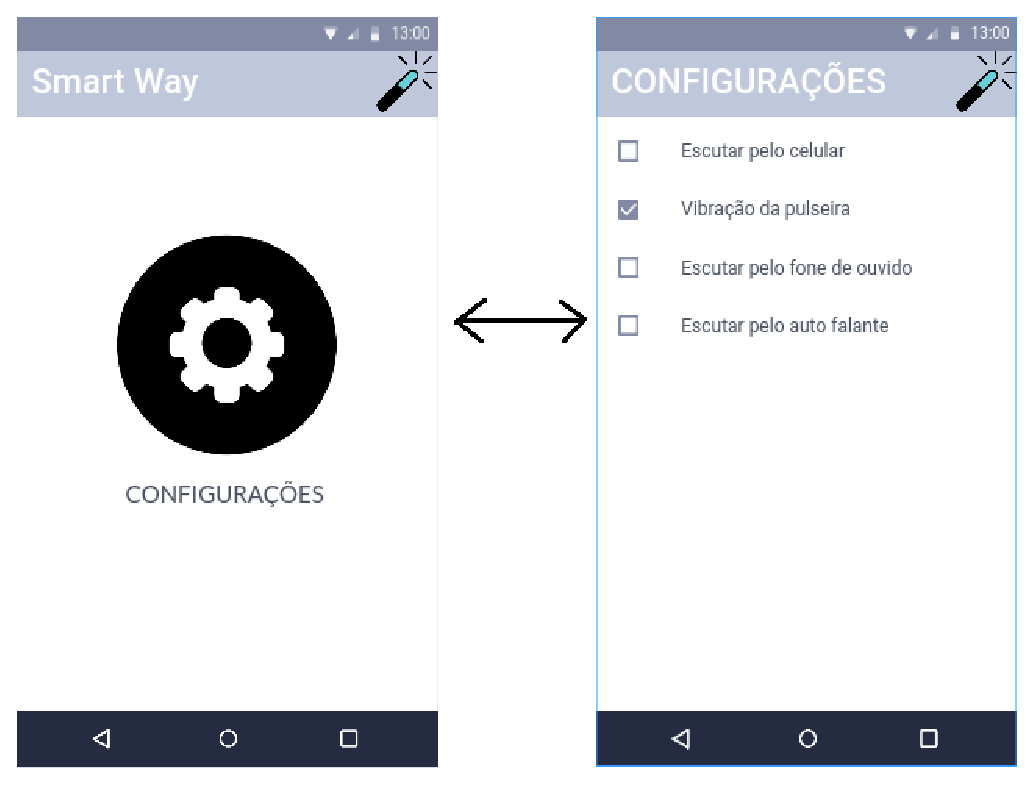
\includegraphics[keepaspectratio=true,scale=0.8]{figuras/app.eps}
    \caption[Aplicativo.]{Aplicativo. Fonte: Autor}
	\label{fig:app}
\end{figure}